%------------------------------------------------------------------------
%Editar Diplomado
\hypertarget{cv:elegirColaboradores}{\section{Elegir Colaboradores}} \label{sec:elegirColaboradores}

	Esta funcionalidad le permitirá asignar a los Colaboradores con los que trabajará en conjunto durante la creación de los elementos de un caso de uso. Cada persona que sea asignada tendrá permisos especiales cuando ingrese al proyecto asignado.

		\subsection{Procedimiento}

			%Pasos de procedimiento
			\begin{enumerate}
	
			\item Oprima el botón \IUAsignar de algún proyecto existente de la pantalla \ref{fig:GestionarProyectosColaborador} ''Gestionar Proyectos de Colaborador''.
		
			\item Se mostrará la pantalla \ref{fig:ElegirColaboradores}
			
			\begin{figure}[htbp!]
				\begin{center}
					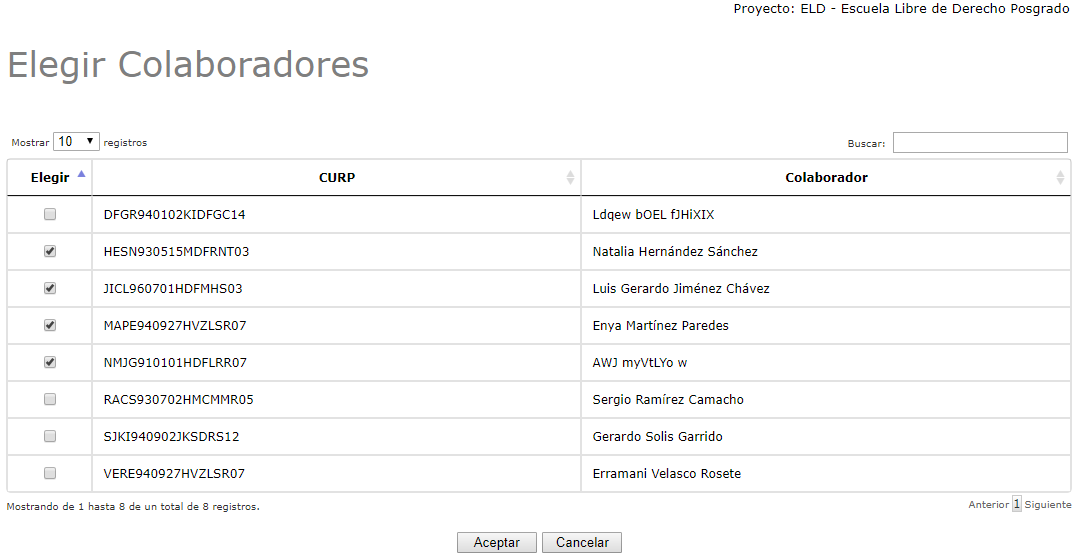
\includegraphics[scale=0.6]{roles/lider/proyectosColaborador/pantallas/IU4-1elegirColaboradores}
					\caption{Elegir Colaboradores}
					\label{fig:ElegirColaboradores}
				\end{center}
			\end{figure}
		
		\item Seleccione el colaborador marcando o desmarcando las casillas de cada registro.
		
		\item Oprime el botón \IUAceptar
		
		\item Se mostrará el mensaje \ref{fig:colaboradorElegido} en la pantalla \ref{fig:GestionarProyectosColaborador} ''Gestionar Proyectos de Colaborador''
						
			\begin{figure}[htbp!]
				\begin{center}
					
\includegraphics[scale=0.6]{roles/lider/proyectosColaborador/pantallas/IU4-1MSG1}
					\caption{MSG: Colaboradores Asignados}
					\label{fig:colaboradorElegido}
				\end{center}
			\end{figure}
			\end{enumerate}